\subsubsection{情報共有}
メモを更新してから,my\_help2hikiの2つのコマンド

\begin{itemize}
\item TARGET --push
\item my\_help --hiki
\end{itemize}
を共に行うと,自分のmy\_helpにあるメモ,サーバのバックアップ,
研究室内のメンバーが見ることのできるwikiの全てが同じ内容になる.
研究室内全員が同じ情報を得ることで,情報を共有するという目標が達成できる.

\subsubsection{memo,hiki,latexの自動変換}
\begin{figure}[htbp]\begin{center}
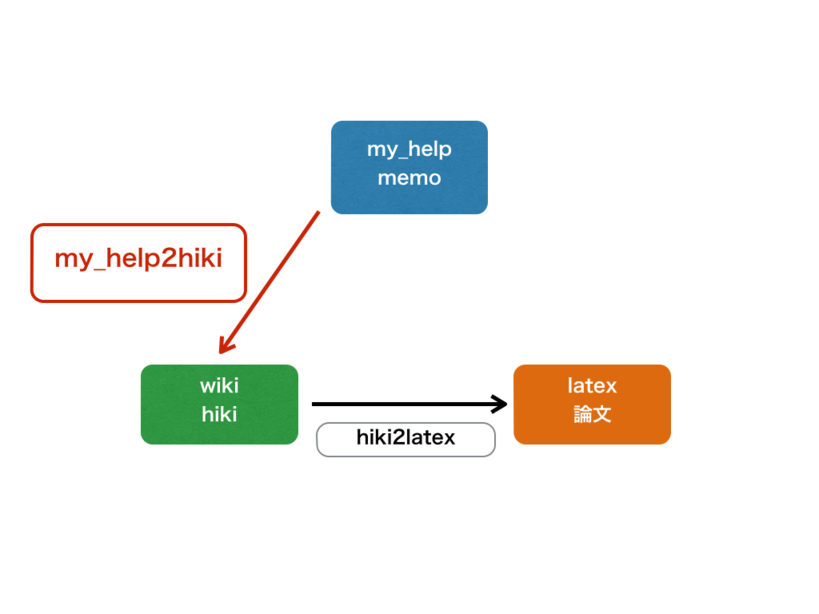
\includegraphics[width=10cm,bb= 0 0 737 453]{../figs/./my_help2hiki_saki.006.png}
\caption{ my\_help2hikiによるmemo,hiki,latexの関係}
\label{default}\end{center}\end{figure}
上記の図のようにmy\_help2hikiを利用することで,memoからwikiを自動変換
が可能になり,my\_helpとhikiの連携ができるようになった.
さらにhiki2latexを利用すればwikiから論文の形のlatexへと変換することもできるので,
研究を進めている際にmemoを作っていれば間接的に,卒業論文へ繋げることができる.

\subsubsection{暗黙知の形式知化}
また,メモをすべてmy\_helpで作成しておけば,忘れてしまったときに
my\_helpのみを確認すればよく,管理も楽になる.
gemの開発中や課題の途中にもすぐメモを残すことができるので,
それぞれのユーザが得た暗黙知もすぐに形式知化することが可能になることが期待される.

